\documentclass[t, mathserif]{beamer}
\usepackage{url}
\usepackage{amsmath}
\usepackage{mathtools}
\usepackage{algorithm} % must read after hyperref
\usepackage{algorithmic}
\usepackage{subfigure,MnSymbol}
\usepackage{graphicx,color,colortbl}
\usepackage{amsfonts,graphics}

\usepackage[normalem]{ulem}
\mode<presentation>
{
  \usetheme{I6pd}
}

\newcommand{\addtext}[4]{\begin{tikzpicture}[overlay,remember picture]
\node[shift={(#3,#4)}]{\color{#1} #2};
\end{tikzpicture}}

% additional packages
\usepackage{times}
%\usepackage{amsmath,amsthm, amssymb, latexsym,MnSymbol}
%\usepackage{exscale}
\usepackage[english]{babel}
\usepackage[latin1]{inputenc}
\usepackage[orientation=landscape,size=custom,width=200,height=120,scale=1.9]{beamerposter}
\graphicspath{{./}{./figures/}}
% Display a grid to help align images
%\beamertemplategridbackground[1cm]
\usepackage[listings,theorems]{tcolorbox}

\title{\huge Efficient Distributed Sensing using Adaptive Censoring-based Inference}
\author[ACL]{Beipeng Mu, Girish Chowdhary, Jonathan P. How}
\institute[LIDS, ACL, MIT]{Laboratory for Information and Decision Systems, 
	Department of Aeronautics and Astronautics,\\ 
	Massachusetts Institute of Technology}
\date[\today]{\today}

% abbreviations
\usepackage{xspace}
\makeatletter
\DeclareRobustCommand\onedot{\futurelet\@let@token\@onedot}
\def\@onedot{\ifx\@let@token.\else.\null\fi\xspace}
\def\eg{{e.g}\onedot} \def\Eg{{E.g}\onedot}
\def\ie{{i.e}\onedot} \def\Ie{{I.e}\onedot}
\def\cf{{c.f}\onedot} \def\Cf{{C.f}\onedot}
\def\etc{{etc}\onedot}
\def\vs{{vs}\onedot}
\def\wrt{w.r.t\onedot}
\def\dof{d.o.f\onedot}
\def\etal{{et al}\onedot}
\makeatother

\iffalse
\newenvironment{mybox}[1]{%
\tcolorbox[savedelimiter=mybox,
savelowerto=\jobname_bspsave2.tex,
lowerbox=ignored,
colback=red!5,colframe=red!75!black,fonttitle=\bfseries,title=#1]}%
{\endtcolorbox}
\begin{mybox}{My Example}
Upper part.
\tcblower
Saved lower part!
\end{mybox}\fi


%%%%%%%%%%%%%%%%%%%%%%%%%%%%%%%%%%%%%%%%%%%%%%%%%%%%%%%%%%%%%%%%%%%%%%%%%%%%%%%%%%%%%%%%%%%%%%%%%%%%%%%%%%%%
%%%%%%%%%%%%%%%%%%%%%%%%%%%%%%%%%%%%%%%%%%%%%%%%%%%%%%%%%%%%%%%%%%%%%%%%%%%%%%%%%%%%%%%%%%%%%%%%%%%%%%%%%%%%
\begin{document}
%\vspace*{.01in}

\begin{frame} 

%\tcbset{width=(\linewidth-60mm)/3,before=,after=\hfill,arc=0mm,
%colframe=blue!75!black,colback=white,fonttitle=\bfseries}
%\begin{tcolorbox}[equal height group=A,adjusted title={One}]
%My smallest box.
%\end{tcolorbox}%
%\begin{tcolorbox}[equal height group=A,adjusted title={Two}]
%This box is also small.
%\tcblower
%But with a lower part.
%\end{tcolorbox}%
%\begin{tcolorbox}[equal height group=A,adjusted title={Three}]
%This box contains a lot of text just to fill the space
%with word flowing and flowing and flowing until the box
%is filled with all of it.
%\end{tcolorbox}\linebreak

% These options will be applied to all `tcolorboxes`
\tcbset{%
    noparskip, %floatplacement=t,float,
    colback=blue!10, %background color of the box
    colframe=structure.fg, %color of frame and title background
    coltext=black, %color of body text
    coltitle=white, %color of title text 
    fonttitle=\bfseries,
		bottom=15mm,top=5mm,boxsep=8mm,left=5mm,right=5mm,arc=8mm, width=.3\textwidth,
boxrule=2mm,before=,after=\hfill,
    white/.style={coltitle=black,colback=white, 
                     colframe=white},
    example/.style={coltitle=black,top=15mm, 
                     colframe=green!20,             
                     colback=green!5},
    }

\begin{tcolorbox}[width=.25\textwidth,after=\hfill,equal height group=A, adjusted title={Distributed Information Fusion Under Uncertainty and Communication Constraints}]
\begin{itemize}
	\item Important to maintain accurate situational awareness for a variety of cooperative multi-agent missions
%For successful completion of cooperative missions by networked systems, maintaining sufficiently accurate
%		situation awareness is essential.
	\begin{itemize}
		\item Key to many other decision making problems, e.g.~distributed planning
		\item Challenging in dynamic, uncertain, communication-constrained environments
		%\item Agents/networks are resource constrained
	\end{itemize}		
\end{itemize}
	\jcols{\bi
		\item \textbf{Problem}: How compute distributed
                  parameter estimates in presence of uncertainties and
                  \alert{communication constraints}? 
		\begin{itemize}
			\item What is correct? \njra centralized Bayesian estimate
			\item Various types of uncertainties
			\item Limited communication/computation resource
		\end{itemize}
	\ei}{
		\begin{figure}[tbh]
			 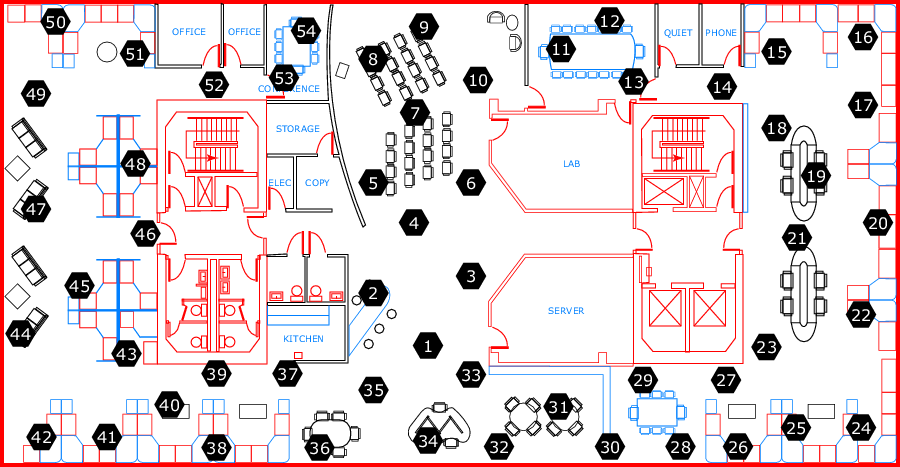
\includegraphics[width=1\columnwidth]{lab.png}

			 \parbox{1\textwidth}{\scriptsize How efficiently handle large
                           data volume collected over distributed nodes?}
		\end{figure}}{.6}{.4}

\begin{itemize}
	\item \textbf{Key features needed:} accurate, scalable, communication efficient
\end{itemize}	
\end{tcolorbox}
% % % % % % % % % % % % % % % % % %
\begin{tcolorbox}[width=.48\textwidth,equal height group=A,adjusted title={Simulation Results},valign=center]
\bi
	\item  Same Poisson arrival rate estimation  on
          slide \ref{slide Poisson}, $V^{\star} \in [0.02,0.5]$
\ei
\vspace{-8mm}
\begin{columns}[T]
\begin{column}{0.45\textwidth}
	\begin{center}
		{\scriptsize Total Communication Cost}
	\end{center}
	\vspace{-8mm}
	\begin{figure}
		 \includegraphics[width=\columnwidth]{cost_VoIDS.png}		 
	\end{figure}
\end{column}
\begin{column}{0.45\textwidth}
%	\vspace{-8mm}
	\begin{center}
		{\scriptsize Cost-Error Summary}
	\end{center}
	\vspace{-8mm}
	\begin{figure}
		\includegraphics[width=\columnwidth]{costError_VoIDS.png}
\addtext{blue}{VoIDS}{-3.5cm}{3cm}
	\end{figure}
\end{column}
\end{columns} 
\bi
  \item  For given $V^{\star}$, comm.\ cost initially grows quickly then levels off
\bii  \item Little known initially, so most new measurements declared informative
\ei
   \item Communication drops in later stages, error cannot be reduced
     further \njra \alert{dynamic} trade-off between cost and accuracy  
  \item How \alert{balance} communication load between early/later stages?
\ei
\end{tcolorbox}
% % % % % % % % % % % % % % % % % %
\begin{tcolorbox}[width=.25\textwidth,equal height group=A,adjusted title={Existing Methods}]
\begin{itemize}	
	\jtem All measurements are broadcast or relayed by all agents to
        all other agents \njra baseline Full-Relay (FR)
		\begin{itemize}
            \item Comparable to centralized Bayesian estimation
			\item Inefficient: communication cost very high (well known)
		\end{itemize}
	\jtem Distributed inference with graphical models~\cite{DurrantWhyte_DataFusion,
  Weiss_BeliefPropagation, bourgault04b, grimeDw94}
		\begin{itemize}
			\item Communication cost lower than FR, can work for arbitrary distributions
			\item Not easily scalable to cyclic graphs
		\end{itemize}
		\jtem Can employ \alert{censoring} 
\begin{itemize}
			\item Differentiate informative measurements from uninformative ones.
			\item Censor uninformative measurements/sensors
		\end{itemize}
   	\jtem Consensus based fusion
		\begin{itemize}
			\item Comm.\ cost lower than FR, but all agents communicate at all times
			\item Dynamic network topology can lead to bias \njra hard to censor agents
		\end{itemize}
	\jtem Random Broadcast (random censoring of agents)
		\begin{itemize}
			\item Communication cost reduced by increasing probability of censoring. \item No bias since all agents have chance to communication
			\item Longer time to convergence since frequency of communication reduced
		\end{itemize}
\end{itemize}
\end{tcolorbox}\\[2ex]

% % % % % % % % % % % % % % % % % %
\begin{tcolorbox}[width=.25\textwidth,after=\hfill,equal height group=B,adjusted title=Our Method: Efficient Distributed Inference]
\begin{itemize}
	\item Value of Information realized Distributed Sensing (VoIDS)
		\bii
			\item Sensors do not communicate measurements all the time
			\item Differentiate between informative and uninformative sensors
			\item Relax restrictions on network topologies 
		\ei


\jtem Will show that this works well, but censoring threshold is somewhat arbitrary and impacts communication cost/performance


	\jtem Developed Adaptive VoIDS (A-VoIDS) \cite{Mu13_Aut}
		\bii
			\item Better balance between communication cost and inference error
		\ei
\end{itemize}
\end{tcolorbox}
% % % % % % % % % % % % % % % % % %
\begin{tcolorbox}[width=.24\textwidth,after=,equal height group=B,adjusted title=Bayesian Update]
\begin{itemize}	
  	\item Bayesian update
%		\begin{varblock}[2.5in]{Bayes Law}
		       $$p (\theta|z,\omega) = \frac { p (z|\theta) p (\theta|\omega)} {\displaystyle \int p(z|\theta) p (\theta|\omega)\,d\theta} $$
%		\end{varblock}
		\bii
			\item $\omega$: hyperparameters of the prior
			\item $\theta$: parameters to be estimated
		\ei
	\jtem Posterior may not have closed form solution
	\jtem Approximate inference methods often used (e.g. Markov Chain Monte Carlo (MCMC) \cite{gelman04}), but still slow and costly
	\jtem In case of exponential family, \alert{closed from solution} exists \njra efficient Bayesian inference
\end{itemize}
\end{tcolorbox}
% % % % % % % % % % % % % % % % % %
\begin{tcolorbox}[width=.24\textwidth,equal height group=B,adjusted title={Exponential Family and Conjugate Prior}]
\begin{itemize}
	\jtem \textbf{Exponential Family}
%		\begin{varblock}[10cm]{}\vspace*{-0.07in}
			$$p(\mathbf{x}|\theta) = \exp\left\{ \theta^T T(\mathbf{x}) - A(\theta)\right\}$$
%		\end{varblock}
		\bii
			\item under measurement $\mu(x)$
			\item $T(\mathbf{x})$: sufficient statistics; $A(\theta)$: log partition
		\ei
	\jtem \textbf{Conjugate prior}
%		\begin{varblock}[10cm]{}\vspace*{-0.07in}
			$$ p(\theta|\omega,\nu) = \exp \left\{ [\omega, \nu]^T [\theta,-A(\theta)] - \Lambda (\omega,\nu) \right\}$$
%		\end{varblock}
		\bii
			\item under measurement $h(x)$
			\item $\omega$, $\nu$: hyperparameters of the prior; $\Lambda$: log partition of conjugate prior
		\ei
%	\jtem \textbf{Posterior}: with new measurements $\mathbf{z}=\{z_i\}_1^n$, the Bayesian posterior has same form as prior; with additive update to hyperparameters 
%		$$\omega \gets \omega+ T(\mathbf{z}),\quad \nu\gets\nu+n$$
%	\jtem  Desired fused estimate of $N$ agent network:
%		$$\omega_{fused}=\omega_0+\sum T(\mathbf{z}),	\quad  \nu_{fused}=\nu_0+\sum n_i$$
\end{itemize}
\end{tcolorbox}
% % % % % % % % % % % % % % % % % %
\begin{tcolorbox}[width=.25\textwidth,equal height group=B,adjusted title=Adaptive VoI Realized Distributed Sensing (A-VoIDS)]
\bi
\item Control frequency of communication by \alertr{adjusting $V^{\star}$ in response to communication load}
\jtem Much better utilization of available communication bandwidth
\bii
\item If many nodes are informative, increase $V^{\star}$  to reduce communication load, 
\item If low communication
    load decrease $V^{\star}$ to increase accuracy
\ei
%    \begin{varblock}[8cm]{Adaptive VoI}
   	$$\begin{array}{l}
 		{V^{\star}} = \left\{ \begin{array}{*{20}{l}}
 		{\gamma _1 V^*} & {\bar{C}[t - l + 1:t] < c}\\
 		{\gamma _2{V^*}} & {\bar{C}[t - l + 1:t] \ge c}	\end{array} \right.\\
 		\gamma _1 > 1, \quad 0< \gamma _2 < 1
 	\end{array}	$$
%    \end{varblock}
        \bii
    	\item $\bar{C}[t - l + 1:t]$: average number of active agents during $[t-l+1:t]$
    	\item $c$: desired communication cost in a step, user-defined
    	\item $\gamma _1$: gaining rate of $V^{\star}$, user-defined
    	\item $\gamma _2$: loosing rate of $V^{\star}$, user-defined
    \ei
\ei
\end{tcolorbox}\\[2ex]

% % % % % % % % % % % % % % % % % %
\begin{tcolorbox}[width=.33\textwidth,equal height group=C,adjusted title={Exponential Family and Conjugate Prior}]
\begin{itemize}
	\jtem brief text
\end{itemize}
\end{tcolorbox}
% % % % % % % % % % % % % % % % % %
\begin{tcolorbox}[width=.33\textwidth,equal height group=C,adjusted title={Summary}]
\begin{itemize}
	\jtem brief text
\end{itemize}
\end{tcolorbox}
% % % % % % % % % % % % % % % % % %
\begin{tcolorbox}[width=.33\textwidth,equal height group=C,adjusted title={Refs}]
\tiny
\bibliographystyle{ieeetr}
\bibliography{../BIB_all/ACL_all,../BIB_all/ACL_Publications,../BIB_all/ACL_bef2000,../BIB_all/bibtex_database_Chowdhary,../BIB_all/bibtex_database_chowdhary_networked}
\end{tcolorbox}

\end{frame}
\end{document}

